\title{Labo: Ontwerp van een audio versterker}
\author{}
\date{}

\documentclass{article}
	\usepackage[a4paper]{geometry}
	\usepackage[utf8]{inputenc}
	\usepackage[T1]{fontenc}
	\usepackage[dutch]{babel}
	\usepackage{amsmath}
	%%% FIGURES %%%
	\usepackage[pdftex]{graphicx}
	\usepackage{caption,subcaption}
	\usepackage{hyperref}
	\graphicspath{ {./figs/} }

\begin{document}
\maketitle
\begin{figure}[htbp]
	\centering
	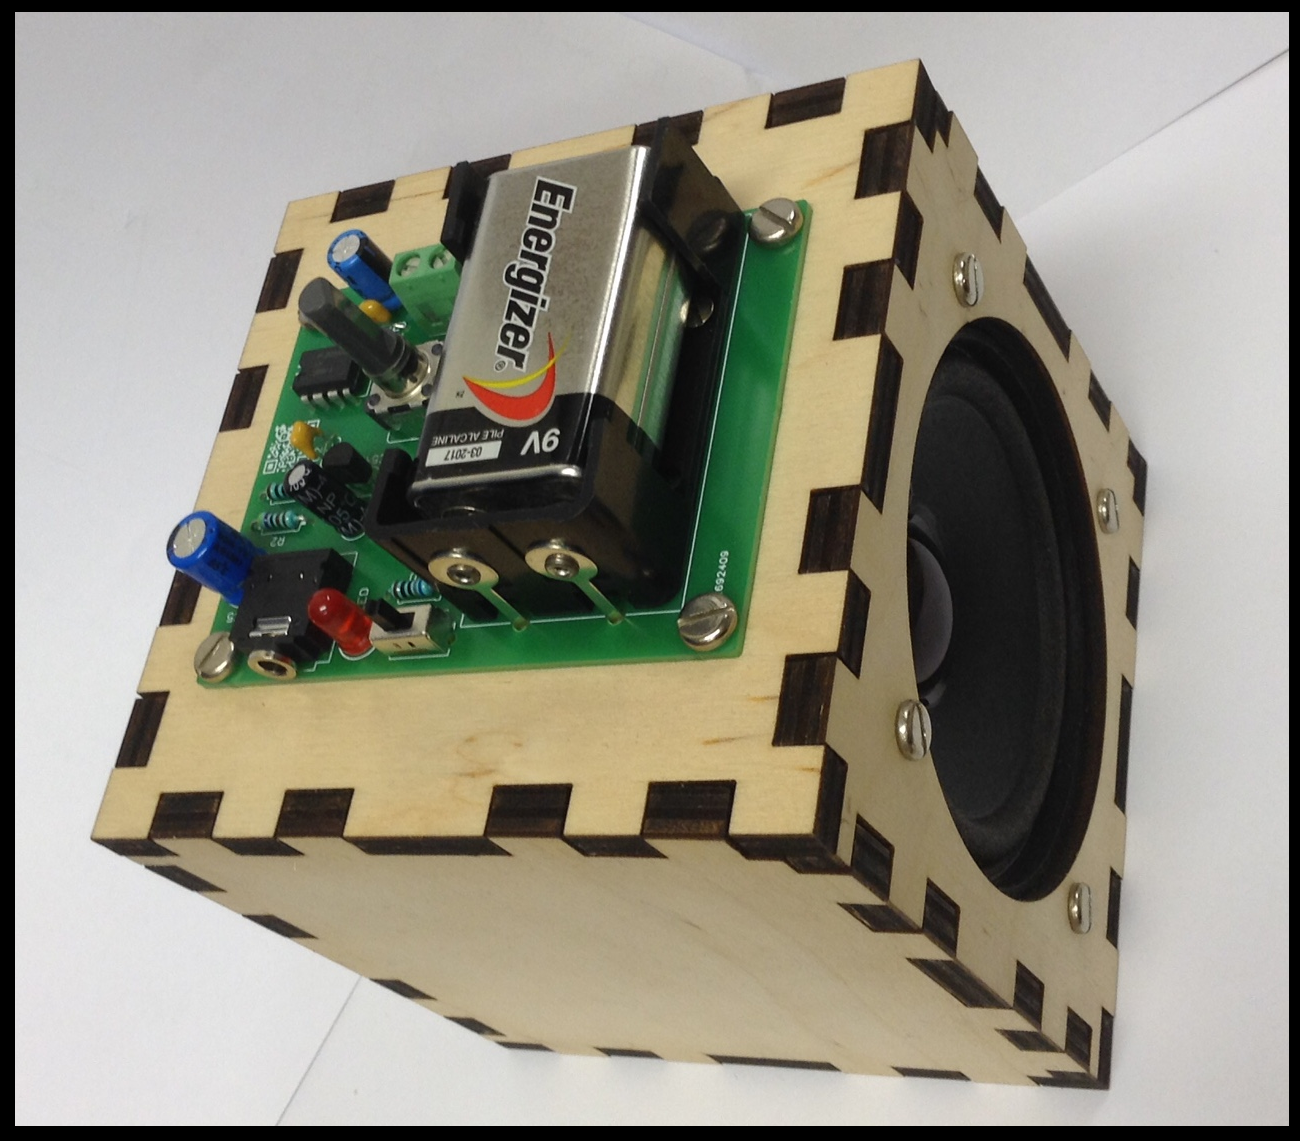
\includegraphics[width=0.4\textwidth]{foto}
	\caption{ E-VUBOX 2k15}
	\label{fig:foto}
\end{figure}
\tableofcontents
\section{Doelstelling}
In dit labo gaan we een eerste stap in de elektronica zetten door zelf een audio versterker te maken, stap voor stap van de basiselektronica tot het finaal product. Tijdens deze opdracht gaan we ook een kijkje nemen in het brein van een ingenieursstudent elektronica wanneer die zo'n taak vervuld. 
beginnen met basis elektronica, kennismaking met basisregels, componenten en schakelingen, naar complexere onderedelen, tot de versterker!

\section{Elektronica: componenten en schakelingen}
Elektronica is het gebruik van de beweging van elektronen om informatie te verwerkern, te versturen of op te slaan. Dit doen we door netwerken van elektronische componenten te bouwen. Elektronische componenten zijn eenvoudige bouwstenen waarmee we complexe schakelingen kunnen bouwen op zo een manier dat die specifieke taken uitvoeren: het ontvangen en versturen van berichtjes met een gsm, het afbeelden van een foto op een scherm en vele andere toepassingen die je elke dag tegenkomt. Je hebt waarschijnlijk een stuk elektronica in jouw broekzak op dit ogenblik!

De schematische voorstelling van elektronische componenten en een netwerk zijn te vinden in Figuur \ref{fig:component_en_schakeling}. Met pijltjes zijn de twee grootheden aangeduid die in de elektronica opperbelangrijk zijn :

\begin{enumerate}
	\item de \textbf{spanning} (of voltage) gemeten in volt [V], vaak aangeduid met de letter $V$ of $U$. Dit stelt het verschil in potentiele elektrische energie \textbf{tussen twee punten}.
	\item de \textbf{stroom} gemeten in ampère [A], vaak aangeduid met de letter $I$. Dit stelt de verplaatsing voor van een hoeveelheid ladingen (hier elektronen) door de component per tijdseenheid.
\end{enumerate}

Stroom en spanning veranderen meestal in functie van de tijd, anders zou er natuurlijk niet veel interessants gebeuren. 

\begin{figure}[hbtp]
	\centering
	\begin{subfigure}[b]{0.45\linewidth}
		\centering
		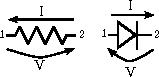
\includegraphics[width=0.8\linewidth]{componenten}
		\caption{Elektronische componenten: een weerstand links en een diode rechts. Men spreekt van de spanning $V$ \textbf{over} de pinnen (1 en 2), en de stroom $I$ \textbf{door} de component. Let op: de zin van de pijlen heeft belang!}
		\label{subfig:componenten}
	\end{subfigure}
	~
	\begin{subfigure}[b]{0.45\linewidth}
		\centering
		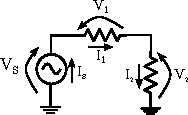
\includegraphics[width=0.8\linewidth]{weerstandsdeler}
		\caption{Elektronisch netwerk: een schakeling van componenten. Er is \textbf{over} elk component een spanningsval , en \textbf{door} elk component een stroom.}
		\label{subfig:netwerk}
	\end{subfigure}
	\caption{Componenten en een schakeling. }
	\label{fig:component_en_schakeling}
\end{figure}
 Elke component voldoet aan fysische wetten die zijn stroom en de spanning bepalen. Laten we kennismaken met die fysiche wetten, en daarna we gaan onmiddelijk ons eerste netwerk oplossen. We bekijken twee basiselementen van de elektronica: de weerstand en de spanningsbron.

\subsection{De weerstand}

In figuur \ref{subfig:componenten} zie je een weerstand (de zaagtand). De weerstand voldoet aan de \textbf{wet van Ohm}: 
\begin{align}
	V &= RI
\end{align} 
$R$ is een eigenschap van de  weerstand die men ook elektrische weerstand noemt, het is gemeten in Ohm\footnote{Georg Simon Ohm (1787 – 1854) was een Duits wiskundige en natuurkundige, ontdekker van de wet van Ohm in 1827.} [$\Omega$]. $V$ is de spanning over de weerstand en $I$ de stroom door de weerstand. Zo dadelijk volgt een voorbeeld, maar we daarvoor moeten we eerst de spanningsbron kennen. 

\subsection{De spanningsbron}

 Een spanningsbron is een simpel elektronisch component die gehoorzaamt aan een eenvoudige wet: de spanningsbron legt de spanning over zijn pinnen vast, onafhankelijk van de rest van het netwerk. Een 9V-batterij is een voorbeeld van een spanningsbron, die de spanning over zijn pinnen vastlegt op constant $9~V$. Een spanningsbron kan een constante spanning opleggen, maar niets verbiedt dat de spanning met de tijd verandert. Beide type bronnen hebben hun eigen schematische voorstelling die je kan vinden in figuur \ref{fig:vbron}.

\begin{figure}[htbp]
	\centering
	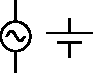
\includegraphics[width=0.1\textwidth]{spanningsbron.pdf}
	\caption{Spanningsbronnen. Links: de spanning verandert met de tijd. Rechts: de spanning is constant.}
	\label{fig:vbron}
\end{figure}

\subsection{Mini-netwerk}
We gaan binnenkort wetten ontdekken van nog meer componenten, maar met onze voorlopige kennis kunnen we al volgend netwerk oplossen!
\paragraph*{Voorbeeld:} 
\begin{figure}[h!]
	\centering
	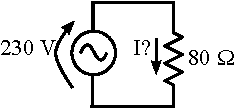
\includegraphics[width=0.25\textwidth]{vbweerstand.pdf}
	\caption{Voorbeeldnetwerkje.}
	\label{fig:vbweerstand}
\end{figure}

Een spanningbron legt een spanning op van $50~V$ over een weerstand van $200~\Omega$. Men kan de stroom door de weerstand berekenen op de volgende manier:

\begin{align}
	\text{(Wet van Ohm)}~V = RI \Leftrightarrow I = \frac{V}{R} \Leftrightarrow I = \frac{50~V}{200~\Omega}= 0,25~A
\end{align}

\paragraph*{Doe-het-zelf:} Wat is de waarde $R$ van een weerstand waarover een spanning van $V = 25~V$ is en waardoor een stroom van $I = 0.1~A$ loopt?
\\.\dotfill \\.\dotfill \\.\dotfill 

Nu we een simpel netwerk kunnen oplossen, gaan we zien hoe we grotere netwerken moeten oplossen.
\subsection{Netwerken}
Een netwerk is een aaneenschakeling van componenten, die schematisch wordt voorgesteld zoals in figuur \ref{subfig:netwerk}. Er zijn maar twee regels die gelden voor elektrische netwerken: de wetten van Kirchoff\footnote{Gustav Robert Kirchhoff (1824–1887) was een Duits natuurkundige. Kirchhoff formuleerde zijn spanningswet en zijn stroomwet in 1845, toen hij nog een student was. Slimme kerel!}. Samen met de fysische wetten van de componenten kan je dan alle netwerken van de wereld oplossen. Een netwerk oplossen wilt zeggen dat je alle stromen en spanningen bepaalt in dat netwerk.

\paragraph*{De stroomwet van Kirchoff:} in elk knooppunt in een elektrische kring is de som van de stromen die in dat punt samenkomen gelijk aan de som van de stromen die vanuit dat punt vertrekken. Dit is voor elk knooppunt geldig, onafhankelijk van de componenten die op de takken zijn. 
\paragraph*{De spanningswet van Kirchoff:} de som van de elektrische potentiaalverschillen (rekening houdend met de richting) in elke gesloten lus in een kring is gelijk aan nul. 

\paragraph*{Voorbeeld}
De stroomwet (figuur \ref{subfig:kcl}) wordt toegepast als volgt: kies een knooppunt in een netwerk. Beschouw alle takken die dat knooppunt raken, en de bijhorende stromen. Pas op, de richting van de pijlen is zeer belangrijk. Als je alle stromen optelt die \textbf{naar} het knooppunt wijzen, dan is dat gelijk aan alle stromen die \textbf{weg} van het knooppunt wijzen.

\paragraph*{}
Voor dat we spanningswet toepassen, hebben we de betkenis van het symbool 
\includegraphics[height=1em]{gnd.pdf} nodig. Dit symbool wordt de \textbf{grond} genoemd. Het is geen component, maar een manier aan te duiden dat alle punten met dat symbool eigenlijk verbonden zijn. Je mag dus eigenlijk een connectie tekenen tussen alle pinnen die aan de grond verbonden zijn. Er werd al gezegd dat een spanning altijd gedifinieerd is tussen twee punten. Meestal wordt de grond gebruikt als een van die twee punten, en we zeggen dat de grond op 0 V is.

\paragraph*{Voorbeeld}
De spanningswet (figuur \ref{subfig:kvl}) vind een gesloten lus in het netwerk (vergeet niet dat alle pinnen aan grond met elkaar verbonden zijn). Teken een lus met een zekere richting in het netwerk. Schrijf de som van de spanningen rekening houdend met de volgende regels:

\begin{enumerate}
 	\item Als de spanning in dezelfde richting gaat als de lus, dan krijgt die een positief teken.
 	\item Als de spanning tegen de lus ingaat, dan krijgt die een negatief teken.
 \end{enumerate}  

\begin{figure}[htbp]
	\centering
	\begin{subfigure}[b]{0.45\linewidth}
		\centering
		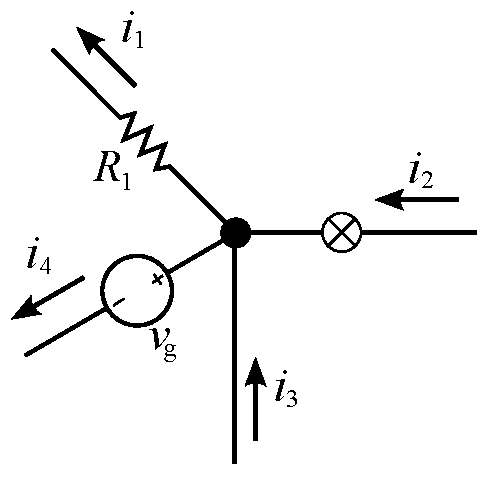
\includegraphics[width=0.7\textwidth]{kcl.pdf}
		\caption{In dit knooppunt is de stroomwet van Kirchoff : $i_1 + i_4 = i_2+i_3$}
		\label{subfig:kcl}
	\end{subfigure}
	~
	\begin{subfigure}[b]{0.45\linewidth}
		\centering
		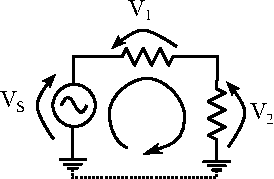
\includegraphics[width=0.8\textwidth]{kvl.pdf}
		\caption{In deze lus is is de spanningswet van Kirchoff : $ + V_S - V_1 - V_2 = 0$}
		\label{subfig:kvl}
	\end{subfigure}
\caption{De wetten van Kirchoff}
\label{fig:kirchoff}
\end{figure}

\begin{itemize}
	\item parallel en serie
	\item weestandsdeler
\end{itemize}


\section{Het nut van een versterker}

Het doel van ons project is om een versterker te bouwen, maar waarom een versterker nodig is wordt hier kort uiteengezet. We willen muziek dat uit onze muziekspeler komt beluisteren. Meestal doen we dat met oortjes of een koptelefoon als we alleen zijn. Maar als we de muziek willen laten beluisteren door vrienden, dan moet het geluid een beetje luider.

Een luidspreker onmiddelijk aansluiten aan onze muziekspeler gaat geen luid lawaai maken. Dit is omdat een luidspreker een hogere spanning en stroom nodig heeft dan wat de muziekspeler kan geven. Dit is waarom een versterker nuttig is, het gaat de spanning aan de uitgang van de muziekspeler versterken en meer stroom kunnen leveren aan de uitgang.

\textbf{Uitleg hoe een luidspreker werkt + muziek is een sinus?}

We weten alles wat nodig is, aan de slag!

\section{Ontwerp}

We gaan nu beginnen met het ontwerp, dat bestaat uit het ingenieus kiezen van de elektronische componenten waaruit de versterker is opgebouwd. Die keuze wordt bepaald door de eisen die we hebben voor de versterker:

\begin{enumerate}
	\item Het ontwerp moet eenvoudig zijn.
	\item De versterker moet draagbaar zijn, om het overal te kunnen gebruiken. ($\rightarrow$ dwz: batterij)
	\item Amplitude van het voltage aan de uitgang van de versterker moet vijf keer groter zijn dan aan de ingang.
	\item De uitgang van de versterker moet genoeg stroom leveren om de luidspreker aan te sturen.
\end{enumerate}

Enkele elektronische ingenieurs zijn ons voorgeweest en hebben al een elektronisch netwerk gemaakt die aan de eisen kan voldoen. Dat netwerk kunnen we vinden in figuur~\ref{fig:volledig_schema}. Dit is een typisch schema dat elektronische ingenieurs gebruiken. 

\begin{figure}[htbp]
	\centering
	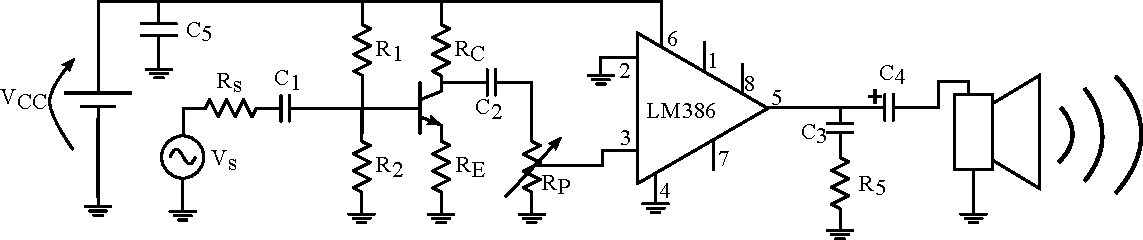
\includegraphics[width=\textwidth]{volledig_schema}
	\caption{Het gebruikt netwerk voor ons ontwerp.}
	\label{fig:volledig_schema}
\end{figure}





\begin{itemize}
	\item serie
	\item parallel
\end{itemize}

\paragraph*{Ons eerst netwerk: de weerstandsdeler}

\begin{itemize}
	\item stroom door R1+R2
	\item spanning over R2
	\item $V_{R2} = \frac{R1}{R1+R2}V$
\end{itemize}
\subsection{Jogging: LED}
\subsection{Eerste Marathon: De Transistor}
\subsection{Tweede Marathon: De Opamp}


\end{document}